\documentclass[letterpaper, 10pt, conference]{ieeeconf}  % Comment this line out if you need a4paper

%\documentclass[a4paper, 10pt, conference]{ieeeconf}% Use this line for a4 paper

\IEEEoverridecommandlockouts                              % This command is only needed if
                                                          % you want to use the \thanks command

\overrideIEEEmargins                                      % Needed to meet printer requirements.

%In case you encounter the following error:
%Error 1010 The PDF file may be corrupt (unable to open PDF file) OR
%Error 1000 An error occurred while parsing a contents stream. Unable to analyze the PDF file.
%This is a known problem with pdfLaTeX conversion filter. The file cannot be opened with acrobat reader
%Please use one of the alternatives below to circumvent this error by uncommenting one or the other
%\pdfobjcompresslevel=0
%\pdfminorversion=4

% See the \addtolength command later in the file to balance the column lengths
% on the last page of the document

% numbers option provides compact numerical references in the text.
% \usepackage{natbib}
\let\proof\relax
\let\endproof\relax
\usepackage{amsthm}
\usepackage{times}
\usepackage{multicol}
\usepackage[bookmarks=true]{hyperref}
\usepackage{xcolor}
\usepackage{hyperref}
\usepackage{amsmath, amssymb}
\usepackage{amsfonts}
\usepackage{graphicx}
\usepackage{siunitx}
\usepackage{standalone}
\usepackage{booktabs}
\usepackage[ruled,vlined,linesnumbered,noend]{algorithm2e}
\usepackage{mdframed}
\usepackage{fancyvrb,multirow}
\usepackage{soul}
\usepackage{dsfont,mathabx}
\usepackage{array, booktabs}
\usepackage{subfigure}
\usepackage{booktabs}
\usepackage{makecell}
\usepackage{threeparttable}
\usepackage{tikz}
\usetikzlibrary{arrows.meta,positioning,fit}
\usetikzlibrary{calc}

%%============================
%%============================

\newtheorem{theorem}{Theorem}
\newtheorem{proposition}{Proposition}
\newtheorem{lemma}[theorem]{Lemma}
\theoremstyle{definition}
\newtheorem{assumption}{Assumption}
\newtheorem{definition}{Definition}
\newtheorem{remark}{Remark}
\newtheorem{example}{Example}
\newtheorem{problem}{Problem}

% GENERAL
\newcommand{\todo}[1]{\textcolor{red}{TODO: #1}}
\newcommand{\improve}[1]{\textcolor{blue}{#1}}
\newcommand{\note}[1]{\textcolor{blue}{NOTE: #1}}
\newcommand{\question}[1]{\textcolor{orange}{Q: #1}}
\newcommand{\change}[1]{\textcolor{black}{#1}}

%%%%%%%%%%%%%%%%%%%%%%%%%%%%%%%%%%%%%%%%%%%%%%%%%%%%%%%
%%%%


\title{\LARGE \bf
  PushAround: Collaborative Path Clearing via \\
  Physics-Informed Hybrid Search
}


% \author{Zili Tang$^1$, Zhongyuan Li$^1$,
%   Zhishao Qiao$^1$ and Meng Guo$^1$ %<-this % stops a space
%   \thanks{The authors are with: $^1$the College of Engineering,
%     Peking University, China;
%     This work was supported by the National Natural Science Foundation
%     of China (NSFC) under grants 62203017, T2121002, U2241214.
%     Contact: {\tt\small meng.guo@pku.edu.cn}.}% <-this % stops a space
% }

\begin{document}
\maketitle
\thispagestyle{empty}
\pagestyle{empty}


%%========================================


%%========================================
\begin{abstract}
In unstructured environments, the passage of large external vehicles is frequently
blocked by movable obstacles, which motivates the deployment of mobile robot teams
to proactively clear traversable corridors. Existing approaches to Navigation Among
Movable Obstacles (NAMO) primarily plan sequences of obstacle manipulations but
typically neglect physical feasibility, overlooking essential factors such as robot
dimensions, mass, applied forces, and the coupled dynamics of pushing. This
limitation often results in strategies that cannot be executed reliably in practice.
A physics-informed framework for collaborative multi-robot pushing is introduced,
enabling the active construction of physically feasible paths. The framework jointly
searches the sequence of obstacles to be displaced, the transit motions of robots
between obstacles, and the contact points and forces required for effective
execution. Core components include a W-Clearance Connectivity Graph (WCCG) for
reasoning about vehicle passage under width constraints, a gap-ranking strategy for
prioritizing obstacle-clearing actions, and a simulation-in-the-loop search to
validate push feasibility. Extensive simulations and hardware experiments
demonstrate robust success, scalability, and efficiency compared to baseline NAMO
methods.
\end{abstract}

%%========================================
\section{Introduction}\label{sec:intro}
In many real-world settings, the passage of large vehicles or transport units is
obstructed by movable obstacles such as pallets, boxes, or equipment, motivating
the deployment of mobile robot teams to actively clear traversable corridors and
enable safe passage. This capability is particularly critical in cluttered and
unstructured environments—warehouses, disaster sites, and dense urban spaces—
where conventional path planning methods assume static obstacles and thus fail
once direct routes are blocked~\cite{liu2023path}. Navigation Among Movable
Obstacles (NAMO) has been studied as a means of creating new routes by pushing,
pulling, or rotating obstacles~\cite{stilman2005navigation}, yet most existing
methods abstract away physical feasibility. Factors such as robot dimensions,
obstacle size and mass, contact geometry, applied forces, and the coupled
dynamics of pushing are typically ignored, producing plans that are geometrically
valid but physically unrealizable. The difficulty is amplified by the fact that
a single large robot is often unable to clear a corridor unaided, smaller robots
are limited by their reach and access to obstacle boundaries, and cooperative
pushing introduces strong physical coupling where one action can trigger chained
motions of multiple obstacles, making prediction and planning substantially more
complex.




\begin{figure}[t!]
  \centering
  \includegraphics[width=\linewidth]{figures/presearch.pdf}% or {presearch.pdf}
  \vspace{-0.2in}
  \caption{
  \textbf{Frontier presearch and gap prioritization.}
  Each panel overlays the WCCG together with the currently selected face (light blue).
  Numbers in \textbf{red} mark the \emph{gap-crossing order} returned by the presearch,
  and numbers in \textbf{blue} indicate the \emph{local ranking} of first-hop gaps on the current face boundary.
  \textbf{Top left/right:} the same scene with start/goal swapped, results in symmetric gap orders with same cost (\(\approx 12.99\)).
  \textbf{Bottom:} a longer map with \(\sim 30\) obstacles, showing a 14-gap sequence with cost \(\approx 40.36\).
  }
  \label{fig:overall}
  \vspace{-0.2in}
\end{figure}

\subsection{Related Work}\label{subsec:intro-related}

Navigation Among Movable Obstacles (NAMO) has been studied as an extension of
motion planning in cluttered environments. Classical methods planned explicit
sequences of obstacle displacements through pushing, pulling, or
rotating~\cite{stilman2005navigation,stilman2007manipulation}, while later work
introduced heuristic search for scalability~\cite{stilman2007manipulation} and
graph- and sampling-based formulations for larger workspaces~\cite{yao2024local}.
Recent efforts extend NAMO to multi-agent settings where teams of robots clear
passages collaboratively~\cite{tang2024collaborative,ren2025search}. However,
most NAMO approaches still idealize robots as point agents with unlimited
actuation and neglect robot size, obstacle mass, and realistic dynamics, which
leads to plans that are geometrically valid but physically unrealizable.

Collaborative pushing has also been widely investigated in multi-robot
manipulation. Foundational studies examined the mechanics of pushing and the
limit surface model~\cite{goyal1989limit,lynch1992manipulation}, while more
recent work addressed force synchronization~\cite{ni2023progressive}, contact
stability and slip margins~\cite{liu2025physics,chen2015occlusion}, and
cooperative transport of large payloads in structured
environments~\cite{ni2024physics,wang2006multi}. Learning-based approaches have
further explored emergent coordination in cluttered
settings~\cite{feng2025learning}. These studies demonstrate effective
multi-robot cooperation but are generally limited to single-object tasks and
assume strict collision avoidance with surrounding obstacles. As a result,
inter-object interactions and the coupled dynamics of multiple movable
obstacles remain largely unaddressed.

Physics-informed planning has emerged to integrate realistic dynamics into
motion generation. Several methods use physics engines to validate candidate
manipulations~\cite{lin2019efficient} or embed contact simulation directly in
the planning loop~\cite{rouxel2024multi}. Other approaches incorporate dynamic
models into planning for non-prehensile manipulation~\cite{zhou2017pushing,hou2020physics}
or apply learning with physics priors and differentiable physics for
contact-rich tasks~\cite{agrawal2016learning,ha2018reinforcement,ni2023progressive,liu2025physics}.
While these approaches highlight the benefits of embedding physical reasoning,
they often decouple high-level planning from low-level feasibility checks or
remain confined to single-object manipulation. Consequently, they do not scale
to collaborative path clearing in cluttered environments with many movable
obstacles.


\begin{figure*}[t!] % 单栏
\centering
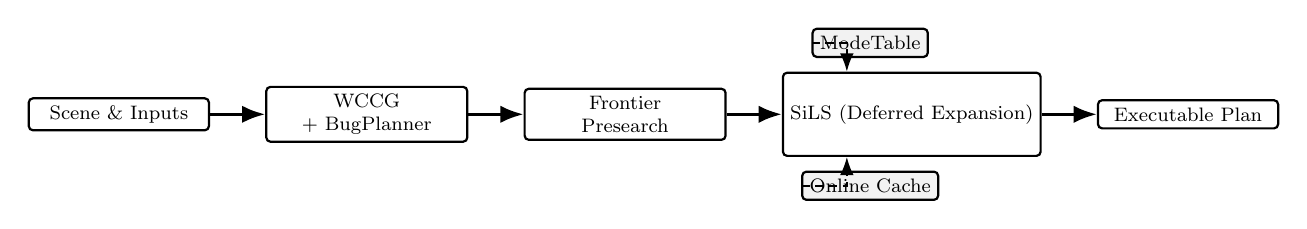
\begin{tikzpicture}[
  scale=0.88, every node/.style={transform shape},
  font=\footnotesize,
  node distance=4mm and 6mm,
  >=Latex,
  box/.style={draw, rounded corners=1.5pt, thick, align=center, inner sep=3pt, fill=white},
  side/.style={box, fill=gray!10},
  line/.style={->, very thick},
  dsh/.style={->, thick, dash pattern=on 3pt off 2pt}
]
\node[box, minimum width=2.6cm] (in)  {Scene \& Inputs};
\node[box, right=8mm of in, minimum width=2.9cm] (wccg) {WCCG\\ + BugPlanner};
\node[box, right=8mm of wccg, minimum width=2.9cm] (pre) {Frontier\\ Presearch};
\node[box, right=8mm of pre, minimum width=3.4cm, minimum height=1.2cm] (sils) {SiLS (Deferred Expansion)};
\node[box, right=8mm of sils, minimum width=2.6cm] (out) {Executable Plan};

% side caches贴在SiLS上方/下方,超短
\node[side, above=2mm of sils, xshift=-6mm] (mt) {ModeTable};
\node[side, below=2mm of sils, xshift=-6mm] (cache) {Online Cache};

\draw[line] (in) -- (wccg);
\draw[line] (wccg) -- (pre);
\draw[line] (pre) -- (sils);
\draw[line] (sils) -- (out);
\draw[dsh] (mt.west) -| ($(sils.north west)!0.5!(sils.north)$);
\draw[dsh] (cache.west) -| ($(sils.south west)!0.5!(sils.south)$);
\end{tikzpicture}
\caption{\todo{Overall framework.}}
\end{figure*}

%==============================
\subsection{Our Method}\label{subsec:intro-our}
This work introduces \emph{PushAround}, a physics-informed framework for
collaborative multi-robot pushing that actively constructs traversable
corridors for large vehicles in cluttered environments. The central novelty is
a hybrid search that jointly determines which obstacles to displace and how to
push them, coupling the high-level sequence of obstacle-clearing actions with
low-level pushing modes that specify contact points, directions, and forces.
The framework integrates three components: a W--Clearance Connectivity Graph
(WCCG) that certifies vehicle passage under width constraints, a gap-ranking
strategy that prioritizes frontier gaps by estimated effort, and a search
procedure that incrementally expands candidate plans while validating their
physical realizability. This integration guarantees that the resulting plans
are not only geometrically valid but also feasible under robot dimensions,
object mass, contact geometry, and coupled pushing dynamics. Efficiency is
achieved by combining compact geometric reasoning with prioritized evaluation,
focusing computation on the most promising actions and avoiding the scalability
issues of simulation-heavy NAMO approaches.

The contributions of this work are twofold: {(I)} it introduces the
first unified framework that couples multi-robot collaborative pushing with
physics-informed feasibility guarantees, producing executable plans for
path clearing in dense cluttered environments; and {(II)} it
demonstrates significant improvements in feasibility, efficiency, and
scalability over existing NAMO and collaborative pushing methods, through
extensive simulation and hardware validation.

%%========================================
%==============================
\section{Problem Description}\label{sec:problem}

%==============================
\subsection{Model of Workspace and Robots}\label{subsec:ws}

Consider a 2D workspace~$\mathcal{W}\subset \mathbb{R}^2$ cluttered with a set of
immovable obstacles~$\mathcal{O}^{\texttt{fix}}$ and a set of~$M>0$ movable obstacles
$\boldsymbol{\Omega}\triangleq\{\Omega_1,\ldots,\Omega_M\}\subset\mathcal{W}$.
Each movable obstacle~$\Omega_m$ is modeled as a rigid polygon of arbitrary shape,
with mass~$\mathsf{M}_m$, inertia~$\mathsf{I}_m$, and frictional parameters~\cite{}.
Its state at time~$t$ is $\mathbf{s}_m(t)\triangleq(\mathbf{x}_m(t),\psi_m(t))$,
and the occupied area is denoted by~$\Omega_m(t)$.

A team of~$N$ robots~$\mathcal{R}\triangleq\{R_1,\ldots,R_N\}$ operates in the workspace.
Each robot~$R_n$ has state $\mathbf{s}_n(t)\triangleq(\mathbf{x}_n(t),\psi_n(t))$
with position and orientation, and occupies region~$R_n(t)\subset\mathcal{W}$.
Robots are equipped with low-level velocity tracking and can apply contact forces
when interacting with obstacles. The free space at time~$t$ is thus
\[
\widehat{\mathcal{W}}(t) \triangleq
\mathcal{W}\backslash \big(\mathcal{O}^{\texttt{fix}}
  \cup \{\Omega_m(t)\}_{m\in\mathcal{M}}
  \cup \{R_n(t)\}_{n\in\mathcal{N}}\big).
\]

%==============================
\subsection{Collaborative Pushing Modes}\label{ss:interaction_mode}

Robots interact with movable obstacles through \emph{pushing modes}.
For an obstacle~$\Omega_m$, a pushing mode is defined as
$\boldsymbol{\xi}_m\triangleq(\xi_m,\mathbf{F}_m,\mathcal{N}_m)$, where
(I)~$\mathcal{N}_m\subseteq\mathcal{N}$ is the subgroup of robots assigned
to push~$\Omega_m$;
(II)~$\xi_m$ specifies the set of contact points
$\mathbf{c}_n\in\partial\Omega_m$ for each robot;
and (III)~$\mathbf{F}_m$ denotes the set of contact forces applied at these points.
The complete set of possible pushing modes is denoted by~$\Xi_m$.
Different pushing modes induce different obstacle motions, depending on
contact geometry, forces, and frictional parameters~\cite{}.

%==============================
\subsection{Problem Statement}\label{subsec:objective}

The goal is to compute a hybrid plan that reconfigures the movable obstacles
so that a collision-free path of width at least~$W>0$ exists between a given
start~$\mathbf{s}^{\texttt{S}}$ and goal~$\mathbf{s}^{\texttt{G}}$.
The plan specifies the sequence of pushing modes, robot assignments, and
corresponding trajectories. Formally:

\vspace{-0.05in}
\begin{equation}\label{eq:problem}
\begin{split}
\underset{\substack{T,\;\{\mathbf{s}_n(t),\,\forall n\},\\
      \{\boldsymbol{\xi}_m(t),\,\forall m\}}}{\textbf{min}} \quad &
  T + \alpha \sum_{t\in\mathcal{T}}
  \sum_{m\in\mathcal{M}}
  \mathrm{J}_m\big(\boldsymbol{\xi}_m(t),\mathbf{S}_{\mathcal{N}}(t),\mathbf{s}_m(t)\big) \\
\textbf{s.t.}\quad &
\exists\;\mathcal{P}_W:\;\mathbf{s}^{\texttt{S}}\leadsto\mathbf{s}^{\texttt{G}}
\;\text{ with clearance }\geq W, \\
& \mathcal{N}_{m_1}(t)\cap\mathcal{N}_{m_2}(t)=\emptyset,\;\forall m_1\neq m_2,\;\forall t,\\
& R_n(t)\cap R_{n'}(t)=\emptyset,\;\Omega_m(t)\cap\Omega_{m'}(t)=\emptyset,\;\forall t,\\
& R_n(t)\subset\widehat{\mathcal{W}},\;\Omega_m(t)\subset\widehat{\mathcal{W}},\;\forall n,m,\;\forall t.
\end{split}
\end{equation}

Here, $T>0$ is the task duration, $\mathcal{T}\triangleq\{0,1,\cdots,T\}$ the
timeline, and $\alpha>0$ balances duration against effort. The cost
$\mathrm{J}_m(\cdot)$ evaluates the feasibility, stability, and control cost of
choosing a particular pushing mode. The clearance constraint ensures that the
final arrangement of obstacles permits a continuous path~$\mathcal{P}_W$ with
width at least~$W$ from start to goal.

%%========================================
% %% ========================================
\section{Proposed Solution}\label{sec:solution}

This section presents a unified framework for collaborative multi-robot pushing.
The approach consists of three main steps. First, a W-Clearance Connectivity Graph
(Sec.~\ref{subsec:wccg}) is constructed to test the existence of a path of width~$W$
and identify frontier gaps when blocked. Second, a gap-ranking strategy
(Sec.~\ref{subsec:gap}) estimates the cost of clearing candidate gaps and
guides robot coordination. Third, a simulation-in-the-loop search
(Sec.~\ref{subsec:simloop}) expands a configuration-space tree while validating
pushing actions through parallel physical simulation. The overall execution flow
and generalizations are summarized in Sec.~\ref{subsec:overall}.

% %% ========================================
%------------------------------
\begin{figure*}[t!]
  \centering
  \includegraphics[width=0.95\linewidth]{figures/presearch.png}% or {presearch.pdf}
  \vspace{-0.15in}
\caption{
Illustration for {the ranking of potential gaps.}
Each panel shows the WCCG with the current face (light blue).
The algorithm (i) extracts the frontier loop from BugPlanner,
(ii) enumerates candidate bridge--bridge gaps on the loop,
(iii) assigns local first-hop ranks (blue numbers),
and (iv) simulates a short presearch to predict the full gap-crossing sequence (red numbers).
\textbf{Top}: start and goal swapped in the same map give symmetric
sequences with cost $12.99$;
\textbf{Right}: a larger map with about 30 obstacles produces a 14-gap sequence
with cost $24.10$.
}
  \label{fig:presearch}
   \vspace{-4mm}
\end{figure*}
%------------------------------
%==============================================
\subsection{W--Clearance Connectivity Graph}\label{subsec:wccg}

The feasibility of routing the vehicle reduces to whether a width-$W$ corridor 
connects $\mathbf{s}_\texttt{V}^{\texttt{S}}$ and $\mathbf{s}_\texttt{V}^{\texttt{G}}$. 
We introduce a W--Clearance Connectivity Graph (WCCG; Fig.~\ref{fig:wccg}) 
that encodes obstacle adjacencies under clearance $W$ and enables fast connectivity queries. 
Constructed directly from geometry (rather than grids/roadmaps), 
it avoids discretization error and remains consistent—crucial because connectivity is checked repeatedly 
during planning.

\subsubsection{Graph Construction}
The WCCG is built by decomposing each movable obstacle
$\Omega_m\in\boldsymbol{\Omega}$ into convex components. From each component
$C$, a centroid node $v_c$ is created. When two components $C_u$ and $C_v$
have closest points $p_u\in C_u$ and $p_v\in C_v$ with distance less than $W$, 
bridge nodes are added at $p_u$ and $p_v$. These bridge nodes are
connected by a bridge--bridge edge, annotated with the corresponding gap width
$w_{uv}\triangleq\|p_u-p_v\|$, and further linked back to their centroids with
centroid--bridge edges. Narrow passages with $w_{uv}<W$ are explicitly marked
as potential bottlenecks. The resulting graph is defined below:
\begin{equation}\label{eq:wccg}
\mathcal{G}_W\triangleq(\mathcal{V},\; \mathcal{E}_c\cup\mathcal{E}_b),
\end{equation}
where $\mathcal{V}$ contains all centroid and bridge nodes;
$\mathcal{E}_c$ is the set of centroid--bridge edges; and $\mathcal{E}_b$ the
set of bridge--bridge edges annotated by widths $w_{uv}$.

\subsubsection{Connectivity Criterion}\label{subsubsec:bugplanner}
Once $\mathcal{G}_W$ has been constructed, connectivity queries can be
performed without explicitly computing a geometric path. A frontier-tracing
procedure, similar to the BugPlanner~\cite{McGuireCroonTuyls2019}, starts from the vehicle start
$\mathbf{s}_\texttt{V}^{\texttt{S}}$, casts a ray toward the goal
$\mathbf{s}_\texttt{V}^{\texttt{G}}$, and explores the encountered loop of
frontier edges. If a valid exit is discovered, the process continues until the
goal is reached; otherwise a blocking cycle is returned. Successful execution
produces a skeleton $\Sigma$, which is an ordered sequence of centroid and
bridge nodes that certifies $\mathbf{s}_\texttt{V}^{\texttt{S}}$ and
$\mathbf{s}_\texttt{V}^{\texttt{G}}$ lie in the same connected face.
Let the $W$--clear free space be
$\mathcal{F}_W\triangleq\mathbb{R}^2\setminus(\mathcal{O}\oplus\mathbb{B}_{W/2})$,
where $\oplus$ denotes Minkowski addition and $\mathbb{B}_{W/2}$ is a closed
disk of radius $W/2$. A complete criterion for existence of a $W$--clear path
$\mathcal{P}^W_\texttt{V}$ is defined as:
\begin{equation}\label{eq:wccg_criterion}
\begin{aligned}
&\exists\,\mathcal{P}^W_\texttt{V}\subset\mathcal{F}_W:\
  \mathbf{s}_\texttt{V}^{\texttt{S}}\leadsto\mathbf{s}_\texttt{V}^{\texttt{G}} \Longleftrightarrow\
  \Big{\{}\mathbf{s}_\texttt{V}^{\texttt{S}},\mathbf{s}_\texttt{V}^{\texttt{G}}
  \ \text{belong to the} \\
  & \text{same face of }\mathcal{G}_W; \;\mathbb{B}_{W/2}(\mathbf{s}_\texttt{V}^{\texttt{S}}),
  \,\mathbb{B}_{W/2}(\mathbf{s}_\texttt{V}^{\texttt{G}})\subset\mathcal{F}_W\Big{\}},
\end{aligned}
\end{equation}
where $\mathbb{B}_{W/2}(\cdot)$ denotes a disk of radius $W/2$ centered at the
argument. This aligns with~\eqref{eq:wclear} for the external vehicle.

\subsubsection{Skeleton to Path}
The skeleton~$\Sigma$, the output of the previous step,
is an ordered sequence of centroid and bridge nodes connected by frontier
edges in $\mathcal{G}_W$. This skeleton serves as a compact certificate that
$\mathbf{s}_\texttt{V}^{\texttt{S}}$ and $\mathbf{s}_\texttt{V}^{\texttt{G}}$
lie in the same connected face. Given as input the skeleton $\Sigma$, together
with $\mathcal{G}_W$, the clearance $W$, and the endpoint disks
$\mathbb{B}_{W/2}(\mathbf{s}_\texttt{V}^{\texttt{S}})$ and
$\mathbb{B}_{W/2}(\mathbf{s}_\texttt{V}^{\texttt{G}})$, the output is an explicit
$W$--clear path $\mathcal{P}^W_\texttt{V}$. This path is constructed by sliding
each skeleton segment along the boundary of the inflated obstacles, offsetting
slightly inward into $\mathcal{F}_W$, and attaching short connectors inside the
endpoint disks. The resulting $\mathcal{P}^W_\texttt{V}$ remains in
$\mathcal{F}_W$, preserves the homotopy of $\Sigma$, and guarantees clearance of
at least $W$.


\begin{remark}\label{remark:wccg}
  The proposed WCCG differs from sampling- and grid-based planners in two key aspects:
  (I) It avoids discretization of $\mathcal{W}$ and is therefore free from
  resolution-induced errors;
  (II) It relies purely on geometry, which makes
queries highly efficient. These two features are crucial, since connectivity
checks and clearance tests are invoked many times within the hybrid
planner described in the sequel. \hfill$\blacksquare$
\end{remark}





%% \begin{algorithm}[t!]
%% \small
%% \caption{BugPlanner for $W$-width connectivity (skeleton witness)}
%% \label{alg:bugplanner}
%% \DontPrintSemicolon
%% \SetKwInOut{Input}{In}\SetKwInOut{Output}{Out}
%% \Input{$\mathbf{s}^{\texttt{S}}$, $\mathbf{s}^{\texttt{G}}$, WCCG}
%% \Output{if connected: skeleton $\Sigma$; else: frontier loop $\mathcal{L}$}
%% $P\leftarrow\mathbf{s}^{\texttt{S}}$, $\Sigma\leftarrow[\ ]$\;
%% \While{true}{
%%   \If{segment $P\mathbf{s}^{\texttt{G}}$ hits no edge}{\Return $\Sigma \cup \{\texttt{straight}(P,\mathbf{s}^{\texttt{G}})\}$}
%%   Build loop $\mathcal{L}$ by angle-follow from the hit edge; append traversed edges to $\Sigma$\;
%%   \If{$\mathrm{parity}(\mathcal{L},\,\mathbf{s}^{\texttt{S}}\mathbf{s}^{\texttt{G}})$ is odd}{\Return $(\emptyset,\mathcal{L})$}
%%   Choose exit $e$ on $\mathcal{L}$ (outward normal $\to\,\mathbf{s}^{\texttt{G}}$); append arc to $\Sigma$; $P\leftarrow e$ (tiny bias)\;
%% }
%% \end{algorithm}

% %% ========================================
%==============================================
\subsection{Ranking of Potential Blocking Gaps}\label{subsec:gap}

When the condition in~\eqref{eq:wccg_criterion} fails, the vehicle cannot
reach~$\mathbf{s}_\texttt{V}^{\texttt{G}}$ from
$\mathbf{s}_\texttt{V}^{\texttt{S}}$ through a $W$--clear path
$\mathcal{P}^W_\texttt{V}$. In this case, the planner must prioritize
\emph{blocking gaps} on the reachable frontier of $\mathcal{G}_W$. The goal of
this module is to provide an ordered list of such gaps, ranked by their
predicted cost to eventually yield a feasible path, which serves
as a critical guidance for the hybrid search in the sequel.

\subsubsection{Frontier Extraction and Candidate Gaps}
A BugPlanner query on $\mathcal{G}_W$, given
$(\mathbf{s}_\texttt{V}^{\texttt{S}},\mathbf{s}_\texttt{V}^{\texttt{G}},W)$,
either confirms connectivity or returns a counter--clockwise frontier loop
$\mathcal{L}$ that separates the two endpoints. The bridge--bridge edges
visible on $\mathcal{L}$ form the first--hop candidate set
$\Gamma_\mathcal{L}\triangleq\{g_1,\cdots,g_K\}$,
where each $g_k$ is a reachable candidate gap. These candidates are the inputs
to the ranking module, while the output will be an ordered list of the same
set sorted by predicted cost.

\subsubsection{Evaluation for Immediate Cost}
Each candidate $g\in\Gamma_\mathcal{L}$ is evaluated by combining the
cost for the robots to reach the gap and the effort required to widen it.
Let $\mathbf{s}_{\mathcal{R}}$ be the current robot positions,
and $\mathbf{o}_g$ as the outside insertion point of gap $g$. The
resulting one--hop cost is given by:
\begin{equation}\label{eq:step_cost}
\mathsf{C}\big(g \mid \mathcal{L}, \mathbf{s}_{\mathcal{R}}\big)
=\lambda_\texttt{t}\,\mathsf{C}_\texttt{t}\!\left(\mathbf{s}_{\mathcal{R}},\mathbf{o}_g\right)
+\lambda_\texttt{p}\,\mathsf{C}_\texttt{p}(g),
\end{equation}
where $\lambda_\texttt{t},\lambda_\texttt{p}>0$ are weighting factors
for the transition and pushing costs, respectively;
function $\mathsf{C}_\texttt{t}(\cdot)$ denotes the collision-free
distance between two points;
and the function~$\mathsf{C}_\texttt{p}(\cdot)$ measures the widening effort,
which increases when the gap is narrower than $W$,
or when the adjacent obstacles are heavier as scaled by the  mass of adjacent movable
obstacles.



\subsubsection{Long-term Cost w.r.t. Goal}
Furthermore, to prioritize gaps closer to the goal, a heuristic is added to the evaluation,
i.e.,
$h(g)=\eta\,\big\|\mathbf{o}(g)-\mathbf{s}_\texttt{V}^{\texttt{G}}\big\|$,
where $\eta>0$ is a scaling constant. Lastly, a short A$^\star$-style presearch virtually crosses
each candidate gap, recomputes the next frontier, and continues for a limited
beam width and depth. The predicted cost-to-connect is given by:
\begin{equation}\label{eq:pred_cost}
\widehat{\mathsf{Cost}}(g)\triangleq
\mathsf{C}\!\big(g \mid \mathcal{L},\mathbf{s}_{\mathcal{R}}\big)
+\!\!\!\sum_{g'\in\Pi^\star(g)}\!\!\!\big{\{}\mathsf{C}(g' \mid \cdot)+h(g')\big{\}},
\end{equation}
where $\Pi^\star(g)$ is the sequence of subsequent gaps discovered after
virtually crossing $g$;
the dots indicate updated inputs along that rollout;
and the scalar score $\widehat{\mathsf{Cost}}(g)>0$ for each candidate gap.
Consequently,
the final output of this module is the ranked list of candidate gaps, i.e.,
$\textsf{Rank}\big(\Gamma_\mathcal{L}\big)
\triangleq \textbf{argsort}_{g\in\Gamma_\mathcal{L}}\widehat{\mathsf{Cost}}(g)$,
which sorts $\Gamma_\mathcal{L}$ in ascending predicted cost. This
ordered set is passed to the hybrid search module, such that only the
promising gaps are expanded first.

\begin{remark}[Practical Improvement]\label{remark:gap}
Efficiency of the above ranking procedure can be improved by
caching frontier loops, storing the transitions
$(\mathcal{L},g)\mapsto\mathcal{L}'$, and accelerating the edge queries with
axis-aligned bounding-box culling. With a small beam width and depth
(typically around $8$), the runtime of ranking remains negligible compared to
the cost of simulation-based validation. \hfill$\blacksquare$
\end{remark}




%% %------------------------------
%% \begin{algorithm}[t]
%% \small
%% \caption{Frontier Presearch for Gap Ranking (compact)}
%% \label{alg:gap-ranking}
%% \DontPrintSemicolon
%% \SetKwInOut{Input}{In}\SetKwInOut{Output}{Out}
%% \Input{$\mathbf{s}^{\texttt{S}}$, $\mathbf{s}^{\texttt{G}}$, WCCG, $\lambda_{\mathrm{trans}}$, $\lambda_{\mathrm{push}}$}
%% \Output{First-hop gaps ranked by predicted cost}
%% $(\mathcal{L},\texttt{conn})\!\leftarrow\!\texttt{BugFrontier}(\mathbf{s}^{\texttt{S}},\mathbf{s}^{\texttt{G}})$;\;
%% \If{\texttt{conn}}{\Return $\emptyset$}
%% $\mathcal{C}\!\leftarrow$ bridge–bridge gaps on $\mathcal{L}$;\;
%% \For{$g\in\mathcal{C}$}{
%%   $J_1\!\leftarrow\!\lambda_{\mathrm{trans}}\mathsf{C}_{\mathrm{trans}}+\lambda_{\mathrm{push}}\kappa(g)[\max(0,W-w(g))+\delta]$;\;
%%   $(\texttt{succ},J_{\mathrm{tail}})\!\leftarrow\!\texttt{PresearchAfter}(g)$;\;
%%   $\widehat{\mathrm{Cost}}(g)\!\leftarrow\!J_1+\big(\texttt{succ}?J_{\mathrm{tail}}:\infty\big)$;\;
%% }
%% \Return $\mathrm{argsort}_{g\in\mathcal{C}}\widehat{\mathrm{Cost}}(g)$ (asc.)\;
%% \end{algorithm}

% %% ========================================
%==============================================
\subsection{Simulation-in-the-Loop Search}
\label{subsec:simloop}

The final step integrates physical feasibility directly into the planning
process through a simulation-in-the-loop search scheme. Unlike pure
graph-based reasoning, which abstracts away dynamics, this method validates
candidate pushing actions by embedding a fast parallelized physics engine
inside the search loop. In this way, both the sequence of obstacle pushes
and their dynamic feasibility are determined consistently, leading to robust
execution in realistic settings. The procedure consists of three phases:
(i) node selection based on a priority queue;
(ii) expansion through candidate pushing actions validated in simulation;
(iii) termination upon reaching a feasible clearance-$W$ path.

%==============================
\subsubsection{Node Representation and Cost}
\label{subsubsec:simloop-node}
Each search node represents the current configuration of movable obstacles
together with the path status between start and goal. Formally, let
$\nu=(\boldsymbol{\Omega}(t),\,\mathcal{P}_W(t))$, where
$\boldsymbol{\Omega}(t)$ is the current set of obstacle states and
$\mathcal{P}_W(t)$ denotes the existence of a clearance-$W$ path in the
WCCG. The cost of a node is defined as
\begin{equation}\label{eq:simloop-cost}
  \mathrm{C}(\nu)\triangleq T(\nu)+\alpha
  \sum_{g\in\mathcal{G}^{\texttt{crit}}(t)} \mathsf{C}(g,t),
\end{equation}
where $T(\nu)$ is the elapsed task duration,
$\mathcal{G}^{\texttt{crit}}(t)$ is the set of critical gaps, and
$\mathsf{C}(g,t)$ is the clearing cost defined in~\eqref{eq:gap-cost}.
This balances planning time against clearing effort.

%==============================
\subsubsection{Simulation-Guided Expansion}
\label{subsubsec:simloop-expansion}
When expanding a node, the planner hypothesizes pushing one of the blocking
obstacles adjacent to a critical gap. Let $\xi=(\mathbf{c},\mathbf{f})$
denote a candidate pushing mode, with contact point $\mathbf{c}\in\partial\Omega_m$
and force $\mathbf{f}\in\mathbb{R}^2$ applied by a subgroup of robots. The
candidate action is validated through a short-horizon simulation
\begin{equation}\label{eq:simloop-dynamics}
  \Omega_m(t+\Delta t) \leftarrow
  \texttt{SimDyn}\big(\Omega_m(t),\xi,\Delta t\big),
\end{equation}
where $\texttt{SimDyn}(\cdot)$ integrates the coupled robot-object dynamics
with contact forces and friction. If the simulated trajectory avoids
collisions and improves the clearance of at least one critical gap, the
resulting state $\boldsymbol{\Omega}(t+\Delta t)$ is inserted into the queue
as a new node.

%==============================
\begin{algorithm}[t]
  \caption{Simulation-in-the-Loop Search (SiLS).}
  \label{alg:SiLS}
  \SetAlgoLined
  \KwIn{Initial obstacle states $\boldsymbol{\Omega}(0)$, start $\mathbf{s}^{\texttt{S}}$, goal $\mathbf{s}^{\texttt{G}}$.}
  \KwOut{Feasible clearance-$W$ plan $\nu^\star$.}
  Initialize priority queue $Q=\{\nu_0\}$ with $\nu_0=(\boldsymbol{\Omega}(0),\emptyset)$;\\
  \While{$Q\neq\varnothing$}{
    \tcc{\textbf{Selection}}
    Pop $\nu^\star=\textbf{argmin}_{\nu\in Q}\{\mathrm{C}(\nu)+\mathrm{H}(\nu)\}$;\\
    Check path existence in $\mathcal{G}^W(t)$; if feasible, return $\nu^\star$;\\
    \tcc{\textbf{Expansion}}
    Identify $\mathcal{G}^{\texttt{crit}}(t)$ from WCCG;\\
    \ForEach{$g\in\mathcal{G}^{\texttt{crit}}(t)$}{
      Generate candidate pushing modes $\xi\in\Xi(g)$;\\
      Simulate next state $\boldsymbol{\Omega}(t+\Delta t)=\texttt{SimDyn}(\Omega_m,\xi,\Delta t)$;\\
      \If{state is collision-free and improves $w(g,t)$}{
        Insert new node $\nu^+$ into $Q$;\\
      }
    }
  }
  Return best $\nu^\star$ if time limit reached;
\end{algorithm}
%==============================

%==============================
\subsubsection{Correctness and Completeness}
\label{subsubsec:simloop-theory}
The simulation-in-the-loop search inherits both correctness and probabilistic
completeness under mild assumptions. First, correctness follows since each
expansion is validated by a dynamics simulator that enforces physical
constraints, guaranteeing that any returned plan is dynamically feasible.

\begin{lemma}[Correctness]\label{lemma:correctness}
Any plan $\nu^\star$ returned by Algorithm~\ref{alg:SiLS} is feasible for the
physical system, as every action has been validated through forward
simulation with collision checking.
\end{lemma}

Completeness is ensured by the hybrid search structure: as long as the set
of pushing modes $\Xi$ is sufficiently rich and the simulation horizon
$\Delta t$ is bounded below, all feasible solutions are eventually explored.

\begin{theorem}[Probabilistic Completeness]\label{thm:completeness-simloop}
  If a clearance-$W$ path exists, Algorithm~\ref{alg:SiLS} finds a feasible
  plan $\nu^\star$ with probability approaching $1$ as the number of node
  expansions tends to infinity.
\end{theorem}

The proofs follow by extending standard arguments from randomized search
algorithms with embedded feasibility oracles, noting that the simulator
acts as a physical feasibility oracle in this case.

% %%========================================
%==============================
\subsection{Overall Analyses}\label{subsec:overall}

\subsubsection{Execution and Online Adaptation}\label{subsec:execute}
The hybrid search outputs a pushing schedule
$\pi=\{\tau_1,\cdots,\tau_K\}$, where each $\tau_k$ specifies a target gap, a
short-horizon velocity $\mathbf{v}_k\triangleq(v_x,v_y,\omega)$, and a contact
mode $\boldsymbol{\xi}_k$. Execution proceeds sequentially under a hybrid
controller alternating between transition and pushing.

During transition, robots plan collision-free paths in the instantaneous
freespace $\widehat{\mathcal{W}}(t)$ to reach designated contact points.
If two paths are imminently head-on, the corresponding contacts are swapped to
avoid deadlock. During pushing, the velocity $\mathbf{v}_k$ is integrated to
generate a short reference trajectory, which is mapped to per-robot contact
states using $\boldsymbol{\xi}_k$. Each robot $R_n$ applies proportional
velocity control:
$\mathbf{v}_n = K_{\!p}(\widehat{\mathbf{p}}^{\,\text{c}}_n-\mathbf{p}^{\text{c}}_n)$,
$\omega_n = K_{\!r}(\widehat{\psi}^{\,\text{c}}_n-\psi^{\text{c}}_n)$,
where $(\widehat{\mathbf{p}}^{\,\text{c}}_n,\widehat{\psi}^{\,\text{c}}_n)$ are
reference states, $(\mathbf{p}^{\text{c}}_n,\psi^{\text{c}}_n)$ are measured
states, and $K_{\!p},K_{\!r}>0$ are control gains. Small offsets are adapted
online to counter yaw drift and maintain stable contact.

Execution is monitored by timeouts during transition and early-stop tests during
pushing. If a push succeeds, execution advances to $\tau_{k+1}$; otherwise,
control is returned to the planner. At a lower rate, the WCCG is rebuilt and
execution terminates once a $W$--clear path $\mathcal{P}^W_\texttt{V}$ connects
$\mathbf{s}_\texttt{V}^{\texttt{S}}$ and $\mathbf{s}_\texttt{V}^{\texttt{G}}$.

\begin{remark}[Endpoint Booster]
The $W$--CCG criterion may be conservative near endpoints. If connectivity holds
but the disks $\mathbb{B}_{W/2}(\mathbf{s}_\texttt{V}^{\texttt{S}})$ or
$\mathbb{B}_{W/2}(\mathbf{s}_\texttt{V}^{\texttt{G}})$ intersect obstacles, a
small set of auxiliary pushes is applied to clear the disks and enable
execution. \hfill$\blacksquare$
\end{remark}


%----------------------------------------------
\subsubsection{Computational Complexity}\label{subsubsec:complexity}
The cost of each node expansion is dominated by simulation of pushing
strategies. Construction of the $W$--clearance graph $\mathcal{G}_W$ and the
associated connectivity tests scale nearly linearly in the number of movable
obstacles $|\boldsymbol{\Omega}|$, while gap ranking by presearch
in Sec.~\ref{subsec:gap} is lightweight as it is limited to a small subset
of frontier gaps. At expansion, only a fraction of the strategies in
$\mathsf{Rank}(\nu)$ survive the geometric quick-pass and early-stop checks,
which shortens the horizon of the simulator calls defined by
$\mathsf{EvalSim}(\cdot)$. Parallel execution of these simulations across multiple
workers reduces the effective cost nearly linearly until communication overhead
is reached. Deferred expansion further improves efficiency by distributing the
evaluation of $\mathsf{Rank}(\nu)$ across iterations, avoiding redundant
restarts and keeping the priority queue focused on promising frontiers.


%----------------------------------------------
\subsubsection{Generalization}\label{subsec:general}
The framework admits several extensions: 
(I) \textit{Heterogeneous teams.} Per-robot gain tuning and robot-specific mode 
priors enable cooperation among diverse robots; 
(II) \textit{Concurrent pushing.} Multi-object mode generation and conflict-aware 
transition planning allow multiple obstacles to be pushed simultaneously; 
(III) \textit{Dynamic environments.} Periodic $W$--connectivity checks and 
on-demand re-planning handle disturbances such as object drift or unmodeled 
contacts during execution.


% %%========================================

%%========================================
% ============================================================
\section{Numerical Experiments}
\label{sec:experiments}
We evaluate the proposed simulation-in-the-loop NAMO planner (SiLS)
in cluttered environments with both movable and immovable obstacles.
All components (W-CCG presearch, frontier extraction, and ModeTable prior)
are integrated as described in Sec.~\ref{sec:system}.
The implementation is in \texttt{Python~3} and simulations are run in
\texttt{PyBullet}~\cite{coumans2019} on a laptop with an Intel
Core i7\textendash1280P CPU. Videos and logs are provided in the
supplementary material.
\begin{figure}
  \centering
  \includegraphics[width=\columnwidth]{figures/straight.pdf}

\caption{SL-Push}
\end{figure}

\begin{figure}
  \centering
  \includegraphics[width=\columnwidth]{figures/Recursive.pdf}
\caption{Rec-NAMO}
\end{figure}



% ========================================
\subsection{Numerical Simulations}
\label{subsec:sim}
% ========================================
\begin{figure}
  
\end{figure}
\subsubsection{\change{Setup}}
\label{subsec:sim-setup}
\change{
The physics step is $\Delta t = 1/120$\,s and the control period is
$1/40$\,s. Robots are disk/box pushers with risk radii consistent with
the $W$-clearance definition. Movable obstacles have masses uniformly
sampled in $[5,15]$\,kg; immovables are modeled with mass $0$.
A trial succeeds when a $W$-clear path from start to goal exists and the
target reaches its goal disc.
}

\paragraph{Workspace and scenarios.}
We use a \emph{nominal scenario} with an $8{\times}5$\,m bounded
workspace, two internal bars (bottlenecks), and a mixed pool of movable
shapes (curved and polygonal, including rings, ellipses, X/T/L/diamond,
arrow-like, rectangles, and cylinders). Two robots start in the lower
left; the target goal lies on the right side. Movables are randomly
placed with a minimum separation. We test \(10\text{--}15\) objects
over multiple seeds.

\paragraph{Geometry and caching.}
Collision checks use polygon/curve-edge models with convex
decomposition when needed. Ray--edge queries for frontiers are
vectorized with AABB culling. Frontier loops are cached by signatures and
transitions $(\mathcal{L},g)\!\mapsto\!\mathcal{L}'$ are memoized.

\subsubsection{\change{Algorithm Configuration}}
\label{subsec:algo-config}
\change{
Unless stated otherwise: per-task simulation horizon $=80$ steps,
up to $64$ candidate push tasks per expansion, and priority
$f = g + \widehat{\mathsf{Cost}}_{\text{to-go}}$ with heuristic factor $10$.
Gap sampling uses a softmax with temperature $0.05$.
ModeTable is enabled (auto-baked if missing).
A \emph{quick-pass} geometry screen may skip physics if a reference
rollout already clears the gap; otherwise a short-horizon simulation with
early stop is used. To avoid premature termination, a
\emph{deferred-reinsertion} rule keeps high-value but temporarily
unexpanded nodes in the queue and revisits them later.
}

\subsubsection{\change{Baselines}}
\label{subsec:baselines}
We compare against three representative families, all using the same
$W$-clearance criterion and contact models:

\begin{itemize}\itemsep2pt
  \item \textbf{DFS-WCCG:} Depth-first search over W-CCG adjacency with
  discrete axis-aligned pushes (object $\times$ \{$\leftarrow,\rightarrow,\uparrow,\downarrow$\}).
  \item \textbf{SL-Push:} Straight-line (or waypointed) route; blockers are
  cleared by (i) off-line minimal normal displacements or
  (ii) sim-in-the-loop normal pushes from near to far.
  \item \textbf{Rec-NAMO:} Recursive routing/pushing on a cost-weighted
  visibility graph: Dijkstra for routing, push-decomposition for local
  clearing; failures prune edges and replan.
\end{itemize}

\subsubsection{\change{Metrics}}
\label{subsec:metrics}
We report success rate, wall-clock time, number of node expansions,
number of simulated pushes, cumulative push time, average presearch
cost-to-go, quick-pass ratio, early-stop ratio, and worker-pool
utilization. Results are averaged over 10 seeds unless noted.

% ==============================
\subsubsection{Main Results}
\label{subsec:main-results}
Table~\ref{tab:main} summarizes performance on the nominal scenario.
SiLS attains higher success with fewer simulations and lower time due to:
(i) frontier-based gap ranking, (ii) ModeTable-guided push directions,
and (iii) quick-pass/early-stop. Deferred reinsertion prevents
priority-queue starvation by revisiting previously generated high-value
nodes when a batch of actions fails.

\begin{table}[t]
  \centering
  \begin{threeparttable}
  \caption{Performance on the nominal scenario with push-count (mean $\pm$ std).}
  \label{tab:main-push}
  \vspace{2pt}
  
  % 🔑 在这里调节列间距
  \setlength{\tabcolsep}{2.3pt} % 默认是 6pt,调小
  
  \begin{tabular}{lccccc}
  \toprule
  Method & Succ.~(\%) & \#PT (s) & \#ET (s) & \#Sims & \#Pushes \\
  \midrule
  DFS-WCCG            & 25 & -- & -- & -- & -- \\
  SL-Push (off-line)  & 62.5 & 0.02 & 145.147 & 0 & 7 \\
  SL-Push (sim)       & 75 & 25.09 & 246.825 & 16 & 8 \\
  Rec-NAMO            & 37.5 & 10.45 & 179.262 & 0 & 7 \\
  \textbf{SiLS (ours)}& \textbf{--} & \textbf{--} & \textbf{--} & \textbf{--} & \textbf{--} \\
  \bottomrule
  \end{tabular}
  
  \begin{tablenotes}[flushleft]\footnotesize
  \item \textbf{Metrics.} \emph{Succ.} = success rate; \emph{\#PT} = planning time; \emph{\#ET} = execution time;
  \emph{\#Sims} = simulations invoked; \emph{\#Pushes} = length of executed push sequence.
  \end{tablenotes}
  \end{threeparttable}
  \end{table}
  


\subsubsection{Ablations}
\label{subsec:ablations}
We remove one component at a time: (i) W-CCG presearch (random gap order),
(ii) ModeTable prior (fallback “away\,+\,jitter” only),
(iii) quick-pass/early-stop (always full physics),
(iv) deferred reinsertion (terminate on empty queue).
Table~\ref{tab:ablation} shows consistent drops in success and increased
time/\#Sims when any component is disabled.

\begin{table}[t]
  \centering
  \caption{Ablations on the nominal scenario (fill with measurements).}
  \label{tab:ablation}
  \vspace{2pt}
  
  % 🔑 调整列间距和行距(只对本表生效)
  {%
  \setlength{\tabcolsep}{3pt} % 列间距缩小
  \renewcommand{\arraystretch}{0.9} % 行距缩小
  
  \begin{tabular}{lcccc}
  \toprule
  Variant & Succ.~(\%) & Time (s) & \#Sims & Quick-pass (\%) \\
  \midrule
  SiLS (full)            & -- & -- & -- & -- \\
  \ \ w/o presearch      & -- & -- & -- & -- \\
  \ \ w/o ModeTable      & -- & -- & -- & -- \\
  \ \ w/o quick-pass/ES  & -- & -- & -- & -- \\
  \ \ w/o reinsertion    & -- & -- & -- & -- \\
  \bottomrule
  \end{tabular}
  }% 局部作用域结束
  
  \end{table}
  

\subsubsection{Efficiency and Scalability}
\label{subsec:eff}
\textbf{Frontier caching} makes BugPlanner near-linear in visible edges.
\textbf{Parallel prediction} uses a persistent worker pool with per-round
broadcast of snapshots and reachable-contact sets to reduce IPC.
\textbf{Quick-pass} and \textbf{early-stop} skip or truncate physics when
geometry suffices. \textbf{Deferred reinsertion} maintains steady depth
growth even when many pushes are rejected.

\subsubsection{Qualitative Results}
\label{subsec:qual}
Figure~\ref{fig:qual} shows a typical run: frontiers and ranked gaps,
a top-ranked gap sequence, simulated pushes that widen bottlenecks, and
the final $W$-clearance path. Per-step overlays and GIFs are produced by
a lightweight snapshot logger.

% \begin{figure}[t]
% \centering
% \includegraphics[width=0.98\linewidth]{figures/qual_demo.pdf}
% \caption{Representative run: frontier (blue), ranked gaps (color-coded by
% predicted cost), simulated pushes (red), and the resulting
% $W$-clearance path (green).}
% \label{fig:qual}
% \end{figure}

\subsubsection{Reproducibility}
\label{subsec:repro}
Random seeds are fixed, JSONL snapshots are logged, and the driver and
scenario generator are released. ModeTable entries are auto-generated if
absent to ensure repeatability across machines.


%%========================================
\section{Conclusion} \label{sec:conclusion}
This work presents a multi-robot framework PushAround for path clearing in unstructured environments using a
hybrid search algorithm that jointly plans obstacles, contact points, and forces with efficiency.
The method demonstrates adaptability to dynamic scenarios. Future directions include estimating
obstacle states without external sensing, addressing uncertain masses, and managing limited robot
visibility to enhance robustness in real-world environments.

%%========================================

\newpage
%========================================
\bibliographystyle{IEEEtran}
\bibliography{contents/references}

\end{document}
